%%%%%%%%%%%%%%%%%%%%%%%%%%%%%%%%%%%%%%%%%%%%%%%%%%%%%%%%%%%%%%%%%%%%%%%%%%%%%%%
\section{Introduction}
%%%%%%%%%%%%%%%%%%%%%%%%%%%%%%%%%%%%%%%%%%%%%%%%%%%%%%%%%%%%%%%%%%%%%%%%%%%%%%%

The Kadomtsev-Petviashvili (KP) equation is a partial differential
equation used to describe the surface height of a two-dimensional
periodic shallow water wave. Depending on certain physical
considerations [XXX], which we will ignore, one can derive either of the
following two equations
\begin{align}
  \left(-4u_t + 6uu_x + u_{xxx}\right)_x + 3\sigma^2 u_{yy} = 0, \quad
  \sigma^2 = -1, \label{eqn: KP1} \\
  \left(-4u_t + 6uu_x + u_{xxx}\right)_x + 3\sigma^2 u_{yy} = 0, \quad
  \sigma^2 = +1. \label{eqn: KP2}
\end{align}
where $u(x,y,t)$ is the surface height as a function of position $(x,y)$
and time $t$. In the sequel we do not rely on this distinction and we
simply refer to the ``KP equation''.

The KP equation admits a large family of quasiperiodic solutions of the
form
\begin{equation} \label{eqn: kpsol}
  u(x,y,t) = 2 \partial_x^2 \log \theta(Ux+Vy+Wt+z_0, \Omega) + c,
\end{equation}
where $\theta$ is the Riemann theta function.

\begin{definition} \label{def: riemanntheta}
  The {\bf Riemann theta function} $\theta: \CC^g \times \hh_g \to \CC$
  is defined in terms of its Fourier series:
  \begin{equation} \label{eqn: riemanntheta}
    \theta(z,\Omega) = \sum_{n \in \ZZ^g}
    e^{2 \pi i \left( \tfrac{1}{2} n \cdot \Omega n + n \cdot z \right)}.
  \end{equation}
  This function converges absolutely and uniformly on compact sets in
  $\CC^g \times \hh_g$ where $\hh_g$ is the space of all {\it ``Riemann
    matrices''} --- complex symmetric matrices with positive definite
  imaginary part.
\end{definition}

From the definition, we see that the Riemann theta function is periodic
in $z$ with integer periods and quasi-periodic in $z$ in the columns of
$\Omega$. In other words, if $m,n \in \ZZ^g$ then
\begin{equation} \label{eq: quasiperiodicity}
    \theta(z + m + \Omega n, \Omega) =
    e^{-2 \pi i \left( \tfrac{1}{2} n \cdot \Omega n + n \cdot z \right) }
    \theta(z, \Omega).
\end{equation}

A generalization of the Riemann theta function, involving a non-integer
shift in some of its arguments, is referred to as the Riemann theta
function with characteristics.

\begin{definition} \label{def: thetachar}
Let $\alpha,\beta \in [0,1)^{g}$. The {\bf Riemann theta function with
characteristic $\thcharsm{\alpha}{\beta}$} is defined as
\begin{align*}
  \theta\thchar{\alpha}{\beta}(z, \Omega) &=
  \sum_{n \in \mathbb{Z}^g}
  e^{2 \pi i \left( \tfrac{1}{2} (n+\alpha) \cdot \Omega (n+\alpha) +
    (n + \alpha) \cdot (z + \beta) \right) } \\
  &=
  e^{2\pi i \left( \tfrac{1}{2} \alpha \cdot \Omega \alpha +
    \alpha \cdot (z + \beta) \right)}
  \theta(z + \Omega \alpha + \beta, \Omega).
\end{align*}
\end{definition}

Note that $\theta \thcharsm{0}{0}(z,\Omega) = \theta(z,\Omega)$. See
\cite{NIST:DLMF,MumfordI07,MumfordII07} for further definitions and
properties of the Riemann theta function.

These soltuions \eqref{eqn: kpsol} are the so-called ``theta function
solutions'' to the KP equation and families of such solutions exist for
every $g > 0$. In fact, the totality of solutions of this form are dense
the space of all periodic solutions to KP \cite{Krichever93}. The
constants $c\in\CC$, $U,V,W,z_0 \in \CC^g$ and $\Omega \in \hh_g$, as
well as the {\it genus} $g$, are determined from a Riemann surface any
such Riemann surface can produce a solution to KP \cite{Dubrovin81}. We
postpone the definition of these constants in terms of known quantities
until more machinery is developed in the following sections.

In general, periodic solutions to integrable partial differential
equations are {\it Abelian functions}.
\begin{definition} \label{def: abelian-function}
  An {\bf Abelian function} $f : \CC^g \to \CC$ of genus $g \geq 1$ is a
  meromorphic function such that there exists $2g$ vectors
  $w_1,\ldots,w_{2g} \in \CC^g$ linearly independent over the real
  numbers where
  \[
      f(z + w) = f(z)
  \]
  for all $z \in \CC^g$. When $g=1$ these are the {\it elliptic
    functions}. The $g \times 2g$ matrix of column vectors $(w_i)$ is
  called the {\it period matrix} of the $f$.
\end{definition}
Abelian functions first arose from the study of Abelian integrals
\[
    \int_{z_0}^{z_1} \frac{P(z,w)}{Q(z,w)}dz
\]
where $P,Q \in \CC[z,w]$ and $z$ and $w$ are related by an algebraic
equation $f(z,w) = 0$ with $f \in \CC[z,w]$. The Jacobi Inversion
Problem is the problem of inverting such integrals, the solution to
which are Abelian functions.

Riemann theta functions play a central role in the theory of Abelian
functions in that all Abelian functions can be written as a rational
function of the Riemann theta function and its derivatives (such as in
the KP solution above).  The primary focus of study is the method of
computation of these Abelian functions, particularly those arising in
applications.

Abelian functions are applicable in fields other than nonlinear partial
differential equations. For example, they make explicit many
computations such as those in the study of solitary waves, black hole
space-times, and algebraic curves. One example in particular is the
calculation of bitangent lines of plane algebraic curves; useful for
computations in optimization-related fields such as algebraic geometry
and convex optimization. In algebraic geometry, bitangents can represent
smooth complex plane quartic curves as both a symmetric determinant of a
linear form (or, determinantal representation) as well as a sum of three
squares \cite{PSV11}. In convex optimization, bitangents are used to
construct a ``visibility complex'' which, in turn, is used to solve the
shortest path problem in Euclidean space \cite{PocchiolaVegter93}.

\begin{definition} \label{def: bitangent}
  A {\bf bitangent} to a plane algebraic curve $C : f(x,y) = 0, f \in
  \CC[x,y]$ is a line $\mathcal{L} \subset \CC$ that lies tangent to $C$
  at at least two distinct points.
\end{definition}

By Bezout's Theorem, if a curve has a bitangent it necessarily must be
of degree at least four \cite{Bezout1779}. A result of Pl\"{u}cker
determines that a degree four complex curve admits exactly 28 complex
bitangents \cite{Plucker34}. In particular, Pl\"{u}cker showed that the
number of real bitangents of any real quartic must be 28, 16, or fewer
than 9. The connection between Riemann theta functions and the bitangent
lines of smooth quartics was known to Riemann \cite{Riemann76,Baker97}
and, in fact, can be computed using the tools developed in this
research. See Figure \ref{fig: edge} for an example.

%% %!!!!!!!!!!!!!!!!
%% %!!!!!!!!!!!!!!!!
%% \marginpar{Note: Figure \ref{fig: edge} will be replaced with the one
%%   generated by abelfunctions once I have it working properly again /
%%   once I find the image on my computer.}
%% %!!!!!!!!!!!!!!!!
%% %!!!!!!!!!!!!!!!!

\begin{figure}[t]
  \centering
  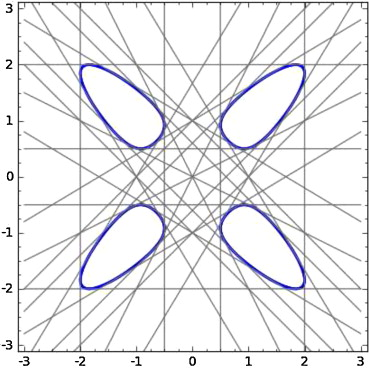
\includegraphics[width=0.6\textwidth]{images/bitangents.jpg}
  \caption{The real graph of the Edge Quartic $C: f(x,y) = 25(x^4+y^4+1)
    - 34(x^2y^2+x^2+y^2) = 0$ (in blue) and its 28 real bitangents (in
    grey). Note that four of them lie tangent $C$ at infinity. These
    lines were computed using the Riemann theta function.}
  \label{fig: edge}
\end{figure}

Finally, Riemann theta functions and algebraic curves can be used to
compute linear matrix representations of algebraic curves. A theorem
from classical algebraic geometry states that every homogenous
polynomial $f \in P^2\CC[x_0,x_1,x_2]$ can be written in the form
\[
   f(x_0,x_1,x_2) = \text{det}
   \left( A x_0 + B x_1 + C x_2 \right),
\]
where $A,B,C$ are symmetric complex matrices which can be efficiently
computed using Riemann theta functions. Furthermore, when the polynomial
has real coefficients then $A,B,C$ are symmetric real matrices and such
representations are important in the study of spectrahedra --- the
solution spaces of semidefinite programs \cite{PSV10}.

The purpose of my research is to develop efficient and performant
algorithms for computing with Abelian functions on Riemann surfaces. The
computational tools developed in this research program have far-reaching
and varied applications.

